\documentclass[../main.tex]{subfiles}

\setlength\parindent{5cm}
\begin{document}
\newpage
\section{Понятия площади и объема. Пути. Термины, связанные с понятием 'путь'. Два подхода к определению кривой, эквивалентные пути. Термины, связанные с понятием 'кривая'.}
\par
Прежде чем определять понятие площади, сначала было бы неплохо поговорить об аддитивной функции промежутка. \\
\[ \Let \left[ A,B\right] \in \R \qquad\Phi:\left\{ \left[ a,b\right]\right\}_{\left[ a,b\right]\in\left[ A,B\right]} \longrightarrow  \R\]
\(\ \Phi\) называется \emph{аддитивной функцией промежутка}, если 
\[ \forall \; a \leq c \leq b: \left[ a,b\right] \subseteq \left[ A,B\right]\quad\Phi \left( \left[ a,b\right]\right)= \Phi \left( \left[ a,c\right]\right)+ \Phi \left( \left[ c, b\right]\right)\]

\begin{examples}
    
    ~

    \begin{enumerate}
        \item \( \Phi \left( \left[ a,b\right]\right)=\left| b-a\right|\) - длина промежутка
        \item \( \Phi \left( \left[ a,b\right]  \right) = \begin{cases}
            1, \text{если } 0 \in \left[ a,b\right)\\ 
            0, \text{если } 0 \notin \left[ a,b\right) 
        \end{cases} \)
        \item \( f \in C\left[ A,B\right],\quad \Phi\left( \left[ a,b\right]\right)= \displaystyle\int\limits_{ a}^{ b} f(x)dx\) \\ Определённый интеграл - аддитивная функция промежутка
    \end{enumerate}
\end{examples}
\[ \Let \; \Phi: \left\{ \left[ a,b\right]\right\}_{ \left[ a,b\right] \subseteq \left[ A,B\right]} \longrightarrow \R,\quad \rho \in C\left[ A,B\right],\quad \forall \; \left[ a,b\right] \subseteq \left[ A,B\right]\quad \Phi \left( \left[ a,b\right]\right)= \displaystyle\int\limits_{ a}^{ b} \rho (x)dx\]
Тогда \( \rho\) называется \emph{плотностью} для \( \Phi \). 
\begin{remark}

    ~

    Не всякая аддитивная функция промежутка имеет плотность. 
    
    Функция из примера 2 плотности не имеет, потому что в интеграле из определения плотности можно зафиксировать нижний предел
    интегрирования. Зафиксируем его равным -10 и будем считать, что \( \Phi\) определена на всех подотрезках отрезка \( \left[ -10, 10\right]\). Тогда \( \forall \;x\in \left[ -10, 10\right]\quad \Phi (\left[ -10,x\right])= \displaystyle\int\limits_{ -10}^{ x} \rho (t)dt\) - 
    это верно из определения плотности. С другой стороны, \( \displaystyle\int\limits_{-10}^{ x} \rho (t)dt\) - это первообразная функции \( \rho\) в точке \( x\) на отрезке \( \left[ -10,10\right]\) по теореме Барроу. Значит первообразная функции \( \rho\) в точке \( x\) равна \( \Phi \left( \left[ -10,x\right]\right)\). Эта первообразная дифференцируема на \( \left[ -10,10\right]\)
    (потому что её производной по определению первообразной должна быть функция \( \rho\)), а значит эта первообразная должна быть непрерывной на \( \left[ -10, 10\right]\). А раз мы знаем, что первообразная функции \( \rho\) в точке \( x\) равна \( \Phi \left( \left[ -10, x\right]\right)\), давайте посмотрим, как ведёт себя \( \Phi\left( \left[ -10,x\right]\right) \).
    На полуинтервале \( \left( -10, 0\right]\) она равна 0, т.к. число 0 не содержится в полуинтервале \(\left[ -10, 0\right)\). На полуинтервале \( \left( 0, 10\right]\quad\Phi \left( \left[ -10, x\right]\right)\) равна 1, т.к. на соответствующих полуинтервалах 0 уже содержится. 
    Получается, что функция \( \Phi \left( [-10,x]\right)\) (которая равна первообразной \( \rho\) в точке \( x\)) имеет разрыв первого рода (скачок) в точке 0, что противоречит тому, что она должна быть непрерывной. 

    То есть чтобы аддитивная функция промежутка имела плотность, необходимо хотя бы чтобы функция \( F(x) = \displaystyle\int\limits_{ x_{ 0}}^{ x} \rho (t)dt\) была непрерывна на \( \left[ A,B\right]\). А какая аддитивная функция промежутка точно имеет плотность? Ответ на 
    этот вопрос даёт признак плотности.
\end{remark}

\begin{thm}[\hypertarget{density_thm}{Признак плотности}]
    
    \( \Let \; \Phi:\left\{ \left[ a,b\right]\right\}_{\left[ a,b\right] \subseteq \left[ A,B\right] } \longrightarrow \R\) - аддитивная функция промежутка,
    \( \rho(x) \in C\left[ A,B\right] \) и
    \[ \forall \;\left[ a, b\right] \subseteq \left[ A,B\right]\quad \min\limits_{ \left[ a,b\right]} \rho \cdot\left( b-a\right) \leq \Phi\left( \left[ a,b\right]\right) \leq \max\limits_{ \left[ a,b\right]} \rho\cdot\left( b-a\right) \]
    Тогда \( \rho(x)\) - плотность \( \Phi\).
\end{thm}
\begin{proof}
    
    ~

    Идея на самом деле в том, что если промежуток \( \left[ a,b\right]\) маленький, то \( \min\limits_{ \left[ a,b\right]} \rho \) и \( \max\limits_{ \left[ a,b\right]} \rho \) это почти одно и то же число, а раз 
    \( \Phi\left[ a,b\right]\) лежит между ними, то ему ничего не остаётся, кроме как равняться им. \( \rho\cdot\left( b-a\right)\) это площадь маленького прямоугольника при близких \( a, b\), а т.к. \( \Phi\) - аддитивная функция промежутка, 
    \( \Phi\left[ a,b\right]\) можно представить в виде суммы её на маленьких отрезках, где она равна площади маленького прямоугольника. А сумма площадей маленьких прямоугольников - это интеграл по Риману.

    \( \Let \; I= \displaystyle\int\limits_{ a}^{ b} \rho(x)dx\), \( X=\left\{ a=x_{ 0},x_{ 1}, \dots,x_{ n}=b\right\}\) - дробление \( \left[ a,b\right]\), \( T = \left\{ t_{ i}\right\}_{i=1}^{n}\) - его оснащение. Вспоминаем определение интеграла по Риману:
    \[ \forall \; \varepsilon >0\quad \exists \; \delta >0:\quad \lambda (X)< \delta \implies \left| I- \sum\limits_{ i=1}^{ n} \rho(t_i) \Delta x_i\right|< \varepsilon \implies I- \varepsilon <\sum\limits_{ i=1}^{ n} \rho\left( t_i\right) \Delta x_i< I+ \varepsilon \]
    Причём это верно для любого оснащения \( T\). Вспомним, что мы умеем оценивать \( \Phi\left( \left[ a,b\right]\right)\).
    \[ \Phi\left( \left[ a,b\right]\right)= \sum\limits_{ k=1}^{ n} \Phi\left( \left[ x_{k-1}, x_k\right]\right) \leq \sum\limits_{ k=1}^{ n} \max\limits_{ \left[ x_{k-1},x_k\right]}\rho\;\cdot \Delta x_k= \sum\limits_{ k=1}^{ n} \rho\left( c_k\right) \Delta x_k\]
    для некоторого \( c_k\in\left[ x_{k-1}, x_k\right]\). Заметим, что \( \sum\limits_{ k=1}^{ n} \rho\left( c_k\right) \Delta x_k\) - это сумма Римана, поэтому \( \sum\limits_{ k=1}^{ n} \rho\left( c_k\right) \Delta x_k < I + \varepsilon \).

    Рассуждая аналогично, \[ \Phi\left( \left[ a,b\right]\right)= \sum\limits_{ k=1}^{ n} \Phi\left( \left[ x_{k-1}, x_k\right]\right) \geq \sum\limits_{ k=1}^{ n} \min\limits_{ \left[ x_{k-1}, x_k\right]} \rho \;\cdot \Delta x_k= \sum\limits_{ k=1}^{ n} \rho\left( \tilde{c_k}\right) \Delta x_k>I- \varepsilon \]

    Таким образом, \[ \forall \; \varepsilon >0\quad I- \varepsilon <\Phi\left( \left[ a,b\right]\right)<I+ \varepsilon \implies \Phi\left( \left[ a,b\right]\right)=I \]
\end{proof}
\emph{Площадь} - неотрицательная функция множества, заданная на некой совокупности множеств \( D(S)\), которые называются \emph{квадрируемыми}. Более полное и подробное определение площади будет дано когда-нибудь позже, когда мы будем разбирать теорию меры, а пока ограничимся этим. \\

{\parindent0pt \textbf{Свойства площади:}}

\begin{enumerate}
    \item \emph{Аддитивность.} Мы привыкли, что площадь аддитивна в том смысле, что если разрезать фигуру на 2 части, то площадь фигуры - это сумма площадей
    обрезков. Но площадь аддитивна ещё и в таком смысле:
    \[ A,B\in D\left( S\right),\quad A \cap B=\varnothing \implies S\left( A \cup B\right)=S\left( A\right)+S\left( B\right)\]
    Это свойство, в частности, позволяет во многих задачах рассматривать площадь как аддитивную функцию промежутка и для её вычисления применять признак плотности. \hyperlink{q15}{Пример можно найти в 15 билете.}
    \item \emph{Инвариантность относительно изометрий (движений).} 
    \[ \Let \;  u: \R^2 \longrightarrow \R^2\quad | \;\forall \;x,y\in\R^2\quad \left| \left| u\left( x\right)-u\left( y\right)\right|\right|=\left| \left| x-y\right|\right| \implies S\left( u\left( A\right)\right)=S\left( A\right)\]  
    Отображение u, удовлетворяющее условию этого утверждения, называется \hypertarget{movement}{\emph{движением}}.
\end{enumerate}

\hyperlink{q14}{Некоторые другие свойства площади рассмотрены в 14 билете}.
\paperline
\emph{Объём} - неотрицательная функция множества, определённая на некотором наборе множеств \( \mathcal{T}\), которые называются \emph{кубируемыми}. 
\[ A,B\in\mathcal{T} \implies A \cup B\in\mathcal{T},\; A\backslash B\in\mathcal{T},\; B\backslash A\in\mathcal{T},\;A \cap B\in\mathcal{T}\]
\begin{prop}{Свойства объёма:}
    Здесь всё по аналогии с площадью.
    \begin{enumerate}
        \item \emph{Аддитивность}\\
        \[T_1, T_2\in\mathcal{T},\quad T_1 \cap T_2= \varnothing \implies V\left( T_1 \cup T_2\right)=V\left( T_1\right)+V\left( T_2\right)\]
        \item \emph{Инвариантность относительно изометрий}\\
        \[ T\in\mathcal{T},\quad \Phi:\R^3 \longrightarrow \R^3\text{ - изометрия} \implies \Phi\left( T\right)\in\mathcal{T},\quad V\left( \Phi\left( T\right)\right)=V\left( T\right)\]
        \item \emph{Нормированность} \\
        Если \( Q\) - прямоугольный параллелепипед со сторонами \( a,b,c\), то \( Q\in\mathcal{T},\quad V\left( Q\right)=abc\).\\ 
        Если при этом одно из чисел \( a,b,c =0\), то параллелепипед называется вырожденным. Обьём такого параллелепипеда равен 0.
    \end{enumerate}
\end{prop} 
\begin{thm}[без доказательства]
    Если \( E\) - квадрируемое плоское множество, \( I =\left[ a,b\right]\) - отрезок, \( C=E\times I\). Тогда \( C\in\mathcal{T},\quad V\left( C\right) = S\left( E\right)\cdot\left( b-a\right)\)
\end{thm}
\begin{note}
    Объём монотонен. 
    \[ A \subseteq B,\quad A,B\in  \mathcal{T} \implies V\left( A\right) \leq V\left( B\right)\]
\end{note}
\begin{proof}
    \[ B \subseteq A \implies B=A \cup \left( B \backslash A\right)\]
    \begin{equation*}
        \begin{aligned}
            &B=A \cup \left( B \backslash A\right)\\
            &A \cap \left( B \backslash A\right)= \varnothing  
        \end{aligned}
        \implies V\left( B\right)=V\left( A\right)+V\left( B \backslash  A\right) \geq V\left( A\right)
    \end{equation*}
\end{proof}
Из этого следует что если \( Q\) - вырожденный параллелепипед, \( E \subseteq Q\), то \( V\left( E\right)=0\)
\begin{thm}[\hypertarget{12_strong_monot}{Усиленная монотонность}]
    \( \Let \; Q\) - вырожденный параллелепипед
    \[ T_1,T_2 \in  \mathcal{T}, \quad T_1 \cap T_2 \subseteq Q \implies V\left( T_1 \cup T_2\right)=V\left( T_1\right)+V\left( T_2\right)\]
\end{thm}
\begin{proof}
    Эта теорема говорит о том, что объём аддитивен не только тогда, когда множества не пересекаются, но и когда множества пересекаются, но немного. Например, два параллелепипеда с общим ребром/гранью.

    \[ T_1 \cap T_2 \subseteq Q \implies V\left( T_1 \cap T_2\right)=0\]
    \begin{equation*}
        \begin{aligned}
            &T_1=\left( T_1 \backslash T_2\right) \cup \left( T_1 \cap T_2\right)\\
            &\left( T_1 \backslash T_2\right) \cap \left( T_1 \cap T_2\right)= \varnothing 
        \end{aligned}
        \implies V\left( T_1\right)=V\left( T_1 \backslash T_2\right)+\underbrace{V\left( T_1 \cap T_2\right)}_0=V\left( T_1 \backslash T_2\right)
    \end{equation*}
    Аналогично \( V\left( T_2\right)=V\left( T_2 \backslash T_1\right)\). \\
    Множества \( T_1 \cap T_2,\; T_1 \backslash T_2,\;T_2 \backslash T_1\) попарно не пересекаются. Кроме того,
    \[ T_1 \cup T_2=\left( T_1 \backslash T_2\right) \cup \left( T_2 \backslash T_1\right) \cup \left( T_1 \cap T_2\right)\]
    Тогда:
    \[ V\left( T_1 \cup T_2\right)=\underbrace{V\left( T_1 \cap T_2\right)}_{0}+V\left( T_1 \backslash T_2\right)+V\left( T_2 \backslash T_1\right)=V\left( T_1 \backslash T_2\right)+V\left( T_2 \backslash T_1\right)=V\left( T_1\right)+V\left( T_2\right)\]
\end{proof}

Некоторые другие свойства объёма описаны в \hyperlink{q16}{16 билете.} 

\paperline

\emph{Путём} в \( \R ^n\) называется отображение \( \gamma \in C\left( \left[ a,b\right] \longrightarrow \R ^n\right),\quad a,b \in \R \).
Такая запись означает, что \( \gamma =\left( \gamma _1, \gamma _2, \dots, \gamma _n\right),\quad \forall \;i\quad \gamma _i \in C\left[ a,b\right]\). При этом \( \gamma _i\left( t\right)\) называется \(i\)-й координатой точки \( t\).

Лучше всего представлять это так, будто аргумент пути \( t\) - это время, а \( \gamma \left( t\right)\) - положение точки в этот момент времени. 

\( \gamma \) называется \emph{гладким}, если \( \forall \;i\quad \gamma _i \in C^1\left[ a,b\right]\). 

Если существует дробление \( \left\{ x_i\right\}_{i=1}^k:\quad \forall \;i=1\dots k\quad \gamma |_{\left[ x_{i-1}, x_i\right]}\) - гладкий путь, то 
\( \gamma \) называется \emph{кусочно-гладким}.

\InsertBoxR{0}{
    \begin{minipage}[t]{6cm} 
        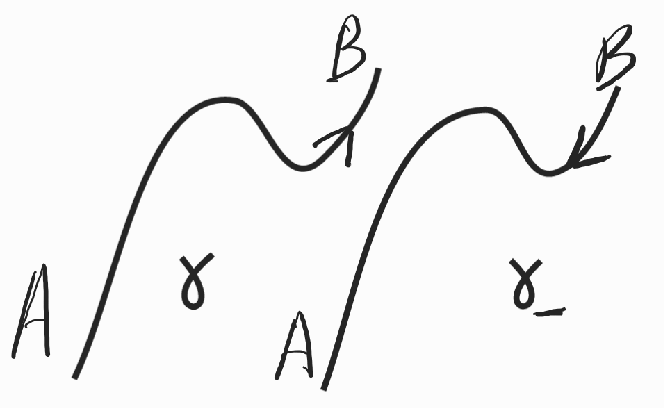
\includegraphics[width=\linewidth]{12_inverse.pdf} 
    \end{minipage}
}

\emph{Носителем пути} называется образ отрезка \( \left[ a,b\right]\) при отображении \( \gamma \).
\( \gamma \left( a\right)\) называется \emph{началом пути}, \( \gamma \left( b\right)\) называется \emph{концом пути}. 

Если \( \gamma :\left[ a,b\right] \longrightarrow \R ^n\) - путь, то отображение \( \gamma _-:\)\[\gamma _-(t)= \gamma \left( a+b-t\right),\quad t \in \left[ a,b\right]\]
называется \emph{противоположным путём} к \( \gamma \). 

~

Если \( \gamma \left( t_1\right)= \gamma \left( t_2\right) \implies t_1=t_2\), то \( \gamma \) называется \emph{простым (Жордановым) путём}. По факту это означает, что 
путь не имеет самопересечений. А если 
\begin{equation*}
    \gamma \left( t_1\right)= \gamma \left( t_2\right) \implies 
    \left[
    \begin{aligned}
        &\;t_1=t_2\\ 
        &\;\left\{ t_1,t_2\right\}=\left\{ a,b\right\}
    \end{aligned}
    \right.
\end{equation*}
то путь называется \emph{простым замкнутым}. То есть он имеет не больше одного самопересечения, которое является его началом и концом. 

~

Под \emph{кривой} часто понимают траекторию простого или простого замкнутого пути. Это первый подход к определению кривой.

Пути \( \gamma : \left[ a,b\right] \longrightarrow \R ^n\) и \( \tilde{ \gamma }: [ \tilde{a}, \tilde{b}] \longrightarrow \R ^n\) называются 
\emph{эквивалентными}, если существует строго возрастающая сюръективная функция \( \varphi :\left[ a,b\right] \longrightarrow [ \tilde{a}, \tilde{b}]\) такая что 
\[ \gamma = \tilde{ \gamma } \circ \varphi \]

\begin{note}
    Это действительно отношение эквивалентности.
    \begin{itemize}
        \item \emph{Рефлексивность:} можно просто взять \( \varphi \) как линейную функцию:
        \[ \varphi = \dfrac{ \tilde{b}-\tilde{a}}{ b-a}\left( x-a\right)+ \tilde{a}\]
        \item \emph{Симметричность:} так как от \( \varphi \) требуется, чтобы оно было строго монотонным, у него точно существует обратное отображение \( \tilde{ \varphi }\), которое тоже будет строго возрастающим. И тогда 
        \[ \tilde{ \gamma }= \gamma \circ \tilde{ \varphi }\]
        \item \emph{Транзитивность:}
        \begin{equation*}
            \begin{aligned}
                &\beta = \alpha \circ \varphi\\
                &\gamma = \beta \circ \chi
            \end{aligned}
            \implies \gamma = \alpha \circ \left( \varphi \circ \chi\right)
        \end{equation*}
        \( \varphi \circ \chi \) - искомое отображение. 
    \end{itemize}
\end{note}

\begin{example}

    ~

    \InsertBoxL{0}{
    \begin{minipage}[t]{7cm} 
        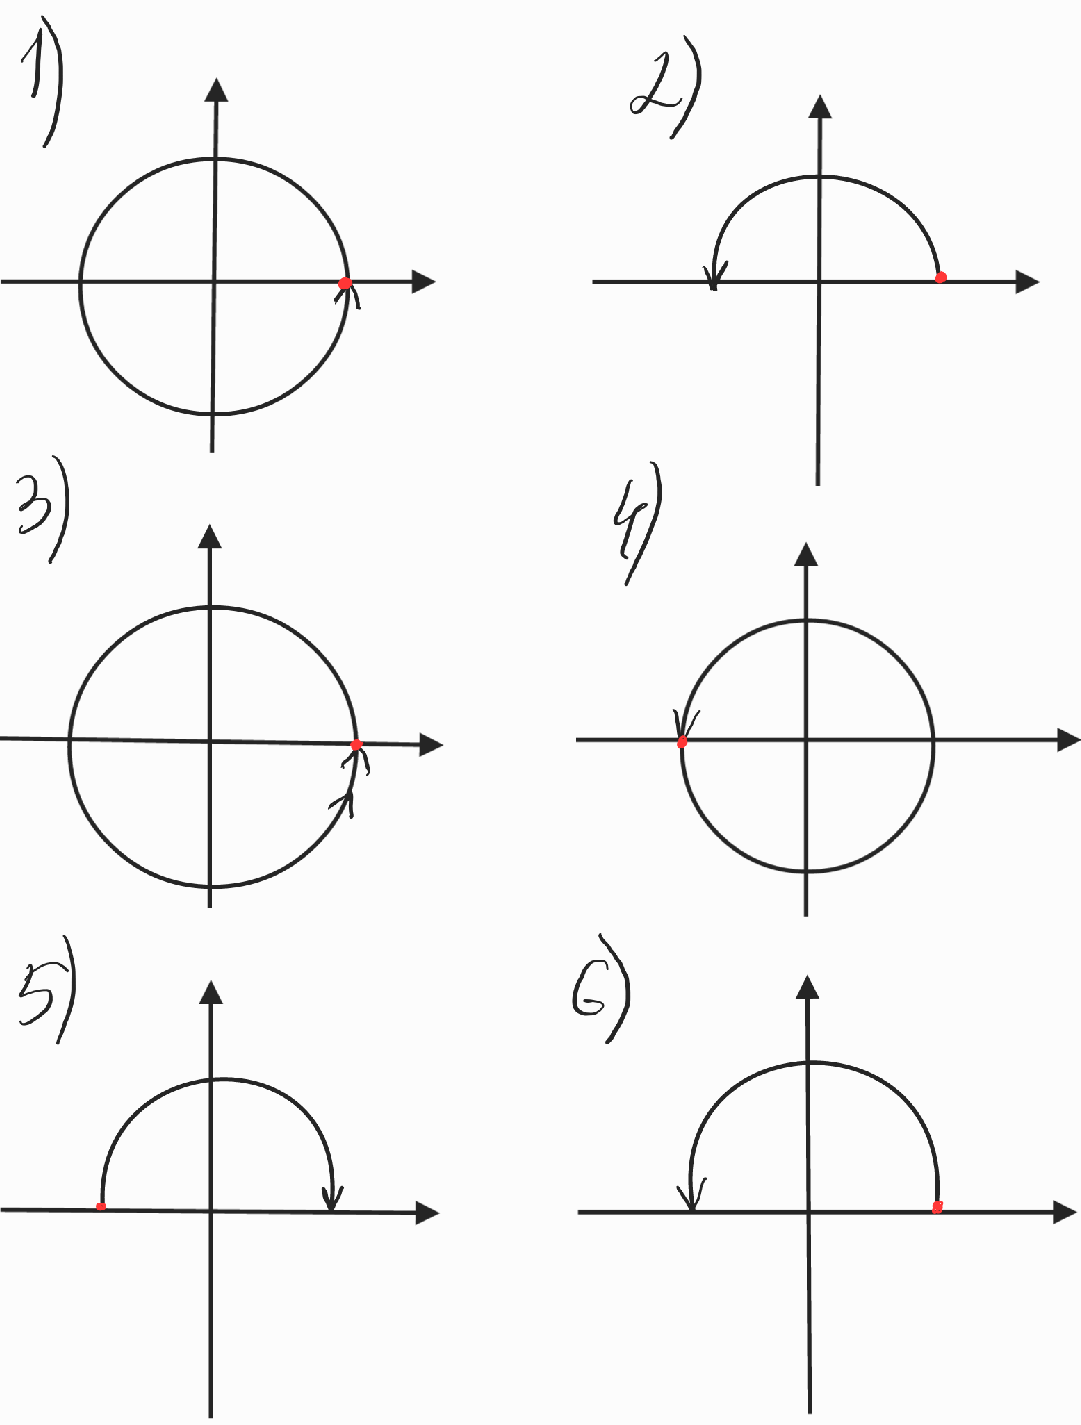
\includegraphics[width=0.9\linewidth]{12_circles.pdf} 
    \end{minipage}
    }
    \begin{equation*}
        \begin{aligned}
            &\gamma _1\left( t\right)= \left( \cos t, \sin t\right),\quad t \in \left[ 0, 2 \pi \right]\\
            &\gamma _2\left( t\right)=\left( \cos t, \sin t\right),\quad t \in \left[ 0, \pi \right]\\
            &\gamma _3\left( t\right)=\left( \cos t, \sin t\right),\quad t \in \left[ 0, 4 \pi \right]\\
            &\gamma _4\left( t\right)=\left( \cos t, \sin t\right),\quad t \in \left[ - \pi , \pi \right]\\
            &\gamma _5\left( t\right)=\left( t, \;\sqrt[]{1-t^2}\right),\quad t \in \left[ -1, 1\right]\\
            &\gamma _6\left( t\right)=\left( -t, \;\sqrt[]{1-t^2}\right),\quad t \in \left[ -1, 1\right]
        \end{aligned}
    \end{equation*}

    Разберём этот пример. Здесь все пути представляют из себя какие-то части окружностей. 
    Сначала нужно понять, что у эквивалентных путей обязательно должны совпадать начало и конец.

    \vspace{15mm}
    ~
     
    Так как отображение \( \varphi \) сюръективно и строго возрастает: 

    \begin{equation*}
        \begin{aligned}
            &\varphi \left( a\right)= \tilde{a}\\
            &\varphi \left( b\right)= \tilde{b}
        \end{aligned}
        \implies 
        \begin{aligned}
            &\gamma \left( a\right)= \tilde{ \gamma }\left( \tilde{a}\right)\\ 
            &\gamma\left( b\right)= \tilde{ \gamma }( \tilde{b}) 
        \end{aligned}
    \end{equation*}

    Таким образом, кандидатами в эквивалентные пути остаются только (1, 3) и (2, 6). Докажем, что если \( \gamma \) простой путь, то эквивалентный ему \( \tilde{ \gamma }\) тоже простой. 

    Пусть \( \gamma \) - простой путь, \( \tilde{ \gamma } \sim \gamma,\quad  \tilde{ \gamma }\left( t_1\right)= \tilde{ \gamma } \left( t_2\right),\quad t_1 \neq t_2\). Тогда 
    \[ \gamma \left( x_1\right)= \tilde{ \gamma }\left( \varphi \left( x_1\right)\right)= \tilde{ \gamma }\left( \varphi \left( x_2\right)\right)= \gamma \left( x_2\right)\]
    при \( \varphi \left( x_1\right) \neq \varphi \left( x_2\right)\). Но \( \varphi \) строго монотонна, а значит инъективна, поэтому \( x_1 \neq x_2\). Итого
    \[ \gamma \left( x_1\right)= \gamma \left( x_2\right),\quad x_1 \neq x_2\]
    чего быть не может по определению простого пути. Аналогично можно получить это утверждение для простого замкнутого пути. 

    Из этого следует, что 1 и 3 не могут быть эквивалентны. Остаются 2 и 6, они действительно эквивалентны, в этом можно убедиться, если в определении эквивалентных путей рассмотреть \( \varphi\left( x\right)=\dfrac{ \pi}{ 2}\left( x+1\right) \).
\end{example}

Если эквивалентность путей - это отношение эквивалентности, то оно должно разбивать множество путей на классы эквивалентности. 

\emph{Второй подход к определению кривой:} если \( \gamma :\left[ a,b\right] \longrightarrow \R \) - путь, то \( \left[ \gamma \right]\) (класс эквивалентности пути \( \gamma \)) называется \emph{кривой}, порождённой \( \gamma \). 
\[ \text{Г}=\left[ \gamma \right]\]
\\
Если Г - кривая, то для любого пути \( \gamma: \left[ \gamma \right]=\text{Г}\quad  \gamma \) называют \emph{параметризацией} Г.
\\
Кривая Г называется \emph{гладкой}, если существует гладкая параметризация Г.
\\
Кривая Г называется \emph{кусочно-гладкой}, если существует кусочно-гладкая параметризация Г.
\\
Кривая Г называется \emph{простой (Жордановой)}, если существует простая параметризация Г.
\\
Кривая Г называется \emph{замкнутой простой}, если существует замкнутая простая параметризация Г.

Если \( \gamma \), заданное на \( \left[ a,b\right]\) - путь и существует дробление \( X=\left( a=x_0, x_1, \dots,x_{n-1}, x_n=b\right)\) отрезка \( \left[ a,b\right]:\quad  \forall \; i=1 \dots n\quad \gamma |_{\left[ x_{i-1 },x_i\right]}\) - аффинная функция (то есть \( \forall \; k=1 \dots n\quad \gamma _k\left( t\right)=kt+b\)), тогда \( \gamma \) называется \emph{ломаной}. 

Некоторые свойства путей, ломаных и кривых рассмотрены в \hyperlink{q13}{13 билете}. 
\end{document}